% rubber: set program xelatex
\documentclass[a4paper,12pt]{article}
\usepackage{xltxtra}
\usepackage{amsmath,amsthm,amssymb}
\usepackage{mathtools}
\usepackage[autostyle=true]{csquotes}
\usepackage{polyglossia}
\setmainlanguage{english}
% Fonts
\setmainfont{CMU Serif}
\setsansfont{CMU Sans Serif}
\setmonofont{CMU Typewriter Text}
\usepackage[xetex, colorlinks=true, citecolor=blue, linkcolor=blue]{hyperref}
\usepackage{fancyhdr} 
\pagestyle{fancy}
\usepackage{graphicx}
\usepackage{placeins}
%\usepackage{subfigure} 
\usepackage{subcaption}
\usepackage{float} 
\usepackage{siunitx}
\usepackage{algorithm}
\usepackage[]{algorithm2e}
% Source code listings
\usepackage{listings}
\usepackage{color}
\usepackage{matlab-prettifier}
\lstdefinestyle{My-Matlab}
{
  style               = MatlabBaseStyle@mlpr,
  basicstyle          = \color{black}\ttfamily\small, 
  mllastelementstyle  = \color{black}                    ,
  mlkeywordstyle      = \color[RGB]{000,000,255}         ,
  mlcommentstyle      = \color[RGB]{034,139,034}         ,
  mlstringstyle       = \color[RGB]{160,032,240}         ,
  mlsyscomstyle       = \color[RGB]{178,140,000}         ,
  mlsectiontitlestyle = \commentStyle@mlpr      \bfseries,
  mlsharedvarstyle    = \color[RGB]{000,163,163}         ,
  mlplaceholderstyle  = \mleditorphstyle,
}
% Commands
\newcommand{\HRule}{\rule{\linewidth}{0.5mm}}
\begin{document}
\begin{minipage}{0.50\textwidth} 
        \begin{flushleft}
        
\includegraphics[scale = 0.50]{Logo-vibot.png}
        \end{flushleft}
\end{minipage}
\begin{minipage}{0.50\textwidth} 
        \begin{flushright}
                
\includegraphics[scale = 0.50]{Logo-ub.png}
        \end{flushright}
\end{minipage}
\begin{center} 
        \vspace*{-1cm}
        \textsc{\Large University of Burgundy}\\[0.5cm]
        \textsc{\Large Masters in Computer Vision}
\end{center}
\vspace*{-0.5cm}
\HRule
\vspace*{4cm}
\begin{minipage}{0.9\textwidth} 
        \begin{center}                                                                                                                                                                  %%%
                \textsc{\LARGE Visual Servoing} \\[0.5cm]
                \textsc{\LARGE \textbf{IBVS \& PBVS \\[0.2cm] Free Camera 3D \\[0.2cm] Pose Control}} \\
                
        \end{center}
\end{minipage}\\[1.5cm]
\begin{center}
{ \Large 
        by \\[0.25cm]
        \textbf{Tsagkatakis Ioannis} \\[1.5cm]
        Under the supervision of \\[0.25cm]
        \textbf{Dr. Omar Tahri} \\
}
\end{center}
\vspace*{2cm}
\begin{center}
        \today
\end{center}
% End First page
\newpage
\tableofcontents 
\section{Introduction}
Visual servo control refers to the use of computer vision data to control  the  motion  of  a  robot. Visual servo control relies on techniques from image processing,  computer  vision,  and  control  theory.   
%We want to move a camera from its current Cartesian pose to a desired Cartesian pose (see Fig. \ref{fig:fig1}). We
%assume that we can measure the Cartesian pose of the camera at every instant of time using a sensor.
%\begin{figure}[H]
%         \centering
%         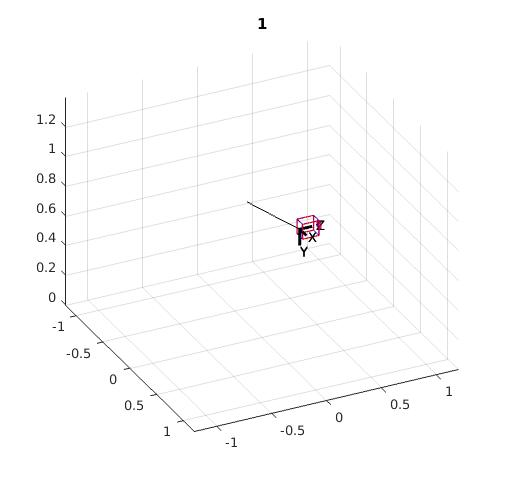
\includegraphics[width=12cm]{../images/pbvs-camera.jpg}
%         \caption{Camera pose control. Blue camera shows the initial pose of the camera, and the red camera shows %the desired pose of the camera.}
%       \label{fig:fig1}
%\end{figure}
\section{The Pose Controll problem}
As the location of the camera is always known we have a Position Based Visual Servoing (PBVS) problem. The control system can be either a real system like a robot or a virtual system like in Viruar Reality applications.
\begin{figure}[b!]
         \centering
         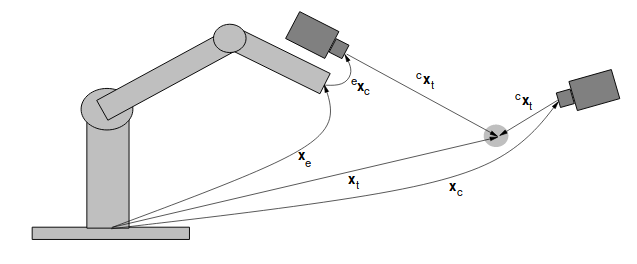
\includegraphics[width=13cm]{coordsys.png}
         \caption{The coordinate frames : word, end-effector, camera and target.}
        \label{fig:coord}
\end{figure}
%% TODO check
The general structure of a PBVS is shown in Figure~\ref{fig:fig2}. A PBVS system operates in Cartesian space and
allows the direct and natural specification of the desired relative trajectories in the Cartesian space.  The parameters extracted from the image $\mathbf{s} = \mathbf{s}(\mathbf{p}_t)$, are used with the models of camera
and object geometry to estimate the relative pose vector $\widehat{\mathbf{W}}$ of the object with respect to the end-effector. The estimated pose is compared with the desired relative pose $\mathbf{W}_d$ to calculate the relative pose error $\widetilde{\mathbf{W}}$.  The coordinate frames involved in the process is given in Figure~\ref{fig:coord} on page~\pageref{fig:coord}.
A Cartesian control law reduces the relative pose error, and the Cartesian control command transformed to 
the joint-level commands for the joint-servo loops by appropriate kinematic transformations.
By separating the pose-estimation problem from the control-design
problem, the control designer can take advantage of well-established robot Cartesian control algorithms.
 
\begin{figure}[tb!]
         \centering
         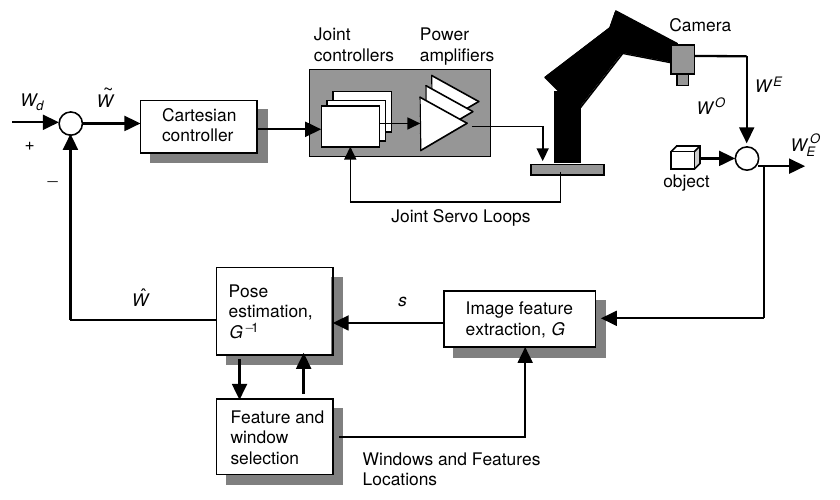
\includegraphics[width=13cm]{../images/PBVS_loop.png}
         \caption{Structure of Position based Visual Servoing (PBVS).}
        \label{fig:fig2}
\end{figure}
\subsection{The Control law}
The visual features parameters extracted from the image are a function of the camera poses as given by
\begin{equation}
        \mathbf{s} = \mathbf{s}(\mathbf{p}_t)
        \label{eq:1}
\end{equation}
By taking the derivative of the above relation we obtain
\begin{equation}
        \dot{\mathbf{S}} = \mathbf{L}_s \mathbf{V} \,\text{,}
        \label{eq:2}
\end{equation}
where $\mathbf{L}_s$ the so called \textit{Interaction matrix} or \textit{feature Jacobian} and $\mathbf{V}$  the 
camera (Kinematic screw) denoted by $\mathbf{V} = \left( \vec{\upsilon}, \vec{\omega} \right)$. Thus thw $\mathbf{V}$ contains 3 translatiosn and 3 rotations. 
The goal of the control law is to minimize the error given by
\begin{equation}
        \mathbf{e}(t) = \mathbf{S}\left(  \mathbf{p}_t \right) -\mathbf{S}^{\ast} \,\text{,}
        \label{eq:3}
\end{equation}
where $\mathbf{S}^{\ast}$ the desired value of the feature.
Using equations \eqref{eq:1} and \eqref{eq:3} then the time variation of the error is
\begin{equation}
        \dot{\mathbf{e}} =  \mathbf{L}_s   \mathbf{V}
        \label{eq:4}
\end{equation}
A good control law is to have an exponential decoupled decrease of the error 
$\dot{\mathbf{e}} = - \lambda\ \mathbf{e}$. 
and we obtain:
\begin{equation}
        \mathbf{V}  =   -\lambda \mathbf{L}_s^+ \mathbf{e}
        \label{eq:4a}
\end{equation}
where $\mathbf{L}_s^+ \in \Re^{6 \times k}$
is  chosen  as  the  Moore-Penrose  pseudoinverse of 
$\mathbf{L}=\left( \mathbf{L}^T \mathbf{L} \right)^{-1} \mathbf{L}^T$, when 
$\mathbf{L}$ is of full rank  6.  
In  real  visual  servo  systems,  it  is  impossible  to  know  perfectly 
in practice either $\mathbf{L}$ or $\mathbf{L}^+$ , so an approximation or an
estimation  $\widehat{\mathbf{L}_s^+}$  must  be  realized.
This corresponds to
\begin{equation}
        \mathbf{V} = -\lambda \widehat{\mathbf{L}_s^+}\left(\mathbf{S}  -\mathbf{S}^{\ast} \right)
        \label{eq:5}
\end{equation}
\subsubsection{Stability analysis}
\begin{equation}
        \begin{cases}
                \widehat{\mathbf{L}_s}\widehat{\mathbf{L}_s^+} = \mathbf{I} 
                        & \text{Ideal behavior} \\
                \widehat{\mathbf{L}_s}\widehat{\mathbf{L}_s^+} >0 & 
                        \text{The error}\, \mathbf{e}\, \text{decreases} \\
                \widehat{\mathbf{L}_s}\widehat{\mathbf{L}_s^+} < 0 & 
                        \text{The error}\, \mathbf{e}\, \text{grows} \\
        \end{cases}
\end{equation}
\section{Image Based Visual Servoing}  
The interaction matrix is given by the equation
\begin{equation}
\begin{bmatrix} 
        -\frac{1}{Z}  & 0 & \frac{x}{Z} & xy & -(1+x^2) & y\\
        0 & -\frac{1}{Z} & \frac{y}{Z} & 1 +x^2 & -x y & -x
\end{bmatrix}
\label{eq:ibvsim} 
\end{equation}
which is a $2 \times 6$ matrix with the first 3 columns corresponds to a translation and the last 3 to a rotation.
\subsection{Algorithm}
\begin{algorithm}[H]
 \While{not at end of time}{
        Build the feature vector $s_A$\\
        Calculate the interaction matrix using \eqref{eq:ibvsim}\\
        Find the error $\mathbf{e}$\\
        Calculate $\widehat{\mathbf{L}_s^+}$ \\
        Calculate the control law
        \begin{equation}
                \xi_{A/R} = 
                \begin{bmatrix}
                        \mathbf{R} & [\mathbf{t}]_{\times} \\
                \mathbf{O}_{3\times 3} & \mathbf{R} \\
                \end{bmatrix}_{A/R} \xi_{A/A}\,,\,
        \xi_{A/A} =
                \begin{bmatrix}
                        v \\ \omega
                \end{bmatrix}
        \end{equation} \\
        Apply the control law and get new camera location \\
 }
 \caption{Image Based Visual Servoing}
\end{algorithm}
\section{Position Based Visual Servoing}  
Let $s(\mathbf{X}) \in \Re^{6 \times 1}$ is a representation of the Cartesian pose  $\mathbf{X} \in \Re^{4 \times 4}$ as follows:
\begin{equation}
        \mathbf{X} =
        \begin{bmatrix}
        \mathbf{R} & \mathbf{t} \\
        \mathbf{0} & 1
        \end{bmatrix}
        \,,\,\,\,
        s(\mathbf{X}) =
        \begin{bmatrix}
        \mathbf{t} \\
        \mathbf{u}\, \theta \\
        \end{bmatrix}\\
        \label{eq:pppbvs}
\end{equation}
where $\mathbf{u}\, \theta $ corresponds to the rotation $\mathbf{R}$. Here $u$ is a unit rotation axis and $\theta$ is the rotation angle around
this axis $\mathbf{u}$. The error can be calculated using the equation
\begin{equation}
        \mathbf{e} = s\left(
        \mathbf{X}_{B/R}^{-1} \star \mathbf{X}_{A(t)/R}
        \right) =
        \mathbf{e} = s\left(
        \mathbf{X}_{A(t)/B}
        \right)
        \label{eq:perror}
\end{equation}
The control law is 
\begin{equation}
        \xi_{A(t)/B} = 
        \begin{bmatrix}
                v \\
                \omega
        \end{bmatrix}_{A(t)/B} =                
        - \lambda 
        \begin{bmatrix}
                \mathbf{R}^t\mathbf{t} \\
                \theta \mathbf{u}
        \end{bmatrix}_{A(t)/B}
        \,\,,\;\; \lambda >0            
                \label{eq:plaw}
\end{equation}
\subsection{Algorithm}
\begin{algorithm}[H]
 \While{not at end of time}{
        Build the feature vector \\
        Find the error $\mathbf{e}$ using equation \eqref{eq:perror}\\
        Calculate $\widehat{\mathbf{L}_s^+}$ \\
        \begin{equation}
                \xi_{A(t)/R} = 
                \begin{bmatrix}
                        \mathbf{R} && [\mathbf{t}_{\times} \mathbf{R} \\
                        \mathbf{0}_{3\times 3} && \mathbf{R}
                \end{bmatrix}_{B/R} \xi_{A(t)/B}
        \end{equation} \\
        Apply the control law and get new camera location \\
        \begin{equation}
                \mathbf{X}_{A(T + \Delta t)/R} = 
                \begin{bmatrix}
                        \Delta t\, [\omega]_{\times} && \Delta t\, v \\
                        \mathbf{0}_{1\times 3} && 1
                \end{bmatrix}_{A(\Delta t)/R} \,
                \mathbf{X}_{A(t)/R}
        \end{equation}
 }
 \caption{Position Based Visual Servoing}
\end{algorithm}
\section{Matlab Experiments}
\subsection{Image Based Visual Servoing}
We want to move a camera from its current location to a desired location relative to a pattern 
(see Figure~\ref{fig:ibvs} on page~\pageref{fig:ibvs})
by using only image point features. We assume that we have only visual feedback. We can take images
and detect image points of the given pattern at 50 Hz. Please do the following exercises:
\begin{figure}[tb!]
         \centering
         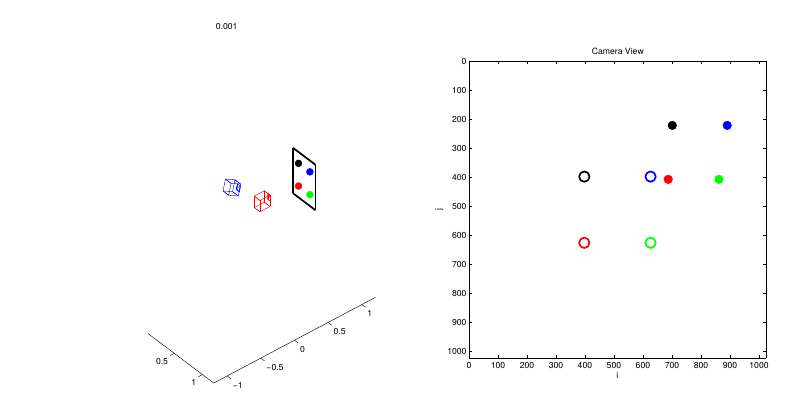
\includegraphics[width=13cm]{../images/IBVS-intro.png}
         \caption{Image based control of the camera pose using point features. Blue camera is the current location,
and the red camera is the desired location of the camera with respect a pattern with four points (left figure).
Empty dots are the desired image points observed from the desired red camera location, and the full dots
are the current image points observed from the current blue camera location (right figure).
.}
        \label{fig:ibvs}
\end{figure}
\subsubsection{A simple example with 4 points}
In the first example we have 2 cameras, and the pattern is clearly visible from them.
\begin{figure}[t!]
                 \begin{subfigure}[b]{\textwidth}         
                \centering
                 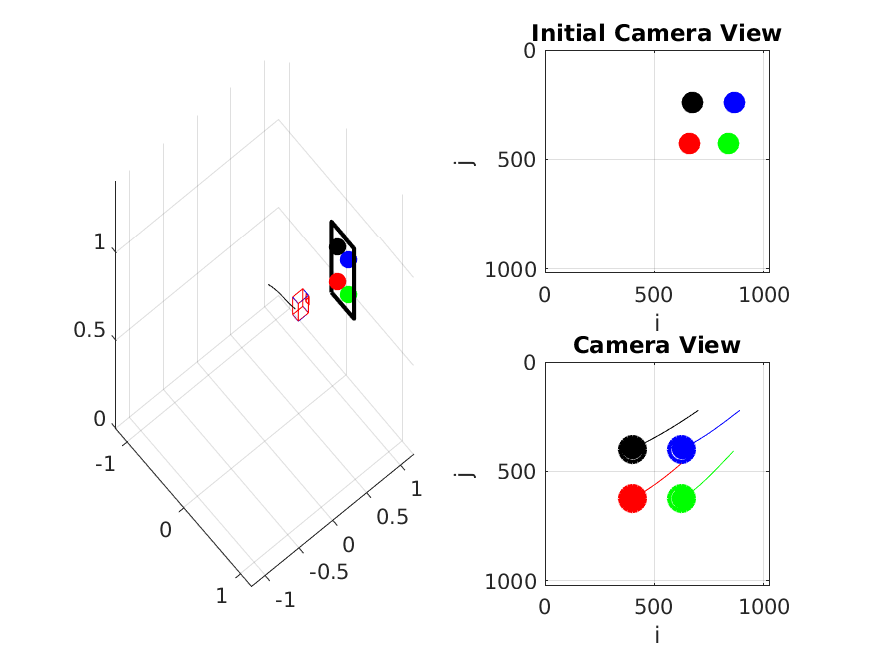
\includegraphics[width=12cm]{../results/Demo1-simulation.png}
             \caption{The camera motion}
             \vspace{8pt}
                 \end{subfigure}
         \begin{subfigure}[b]{0.32\textwidth}
                \centering
                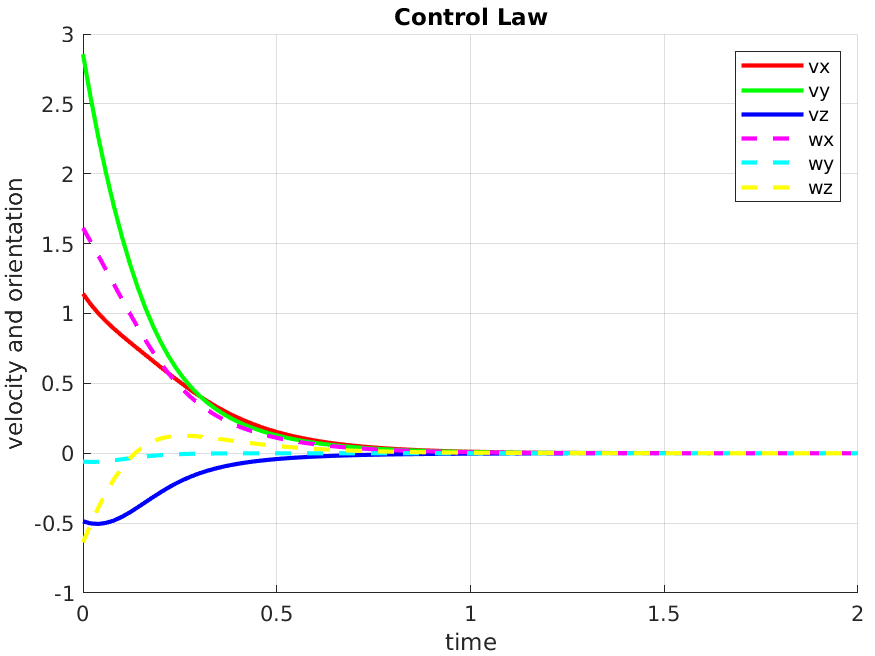
\includegraphics[height=1.2in]{../results/Demo1-control-law.png}
            \subcaption{Control Law}
                 \end{subfigure}
         \begin{subfigure}[b]{0.2\textwidth}
                \centering
                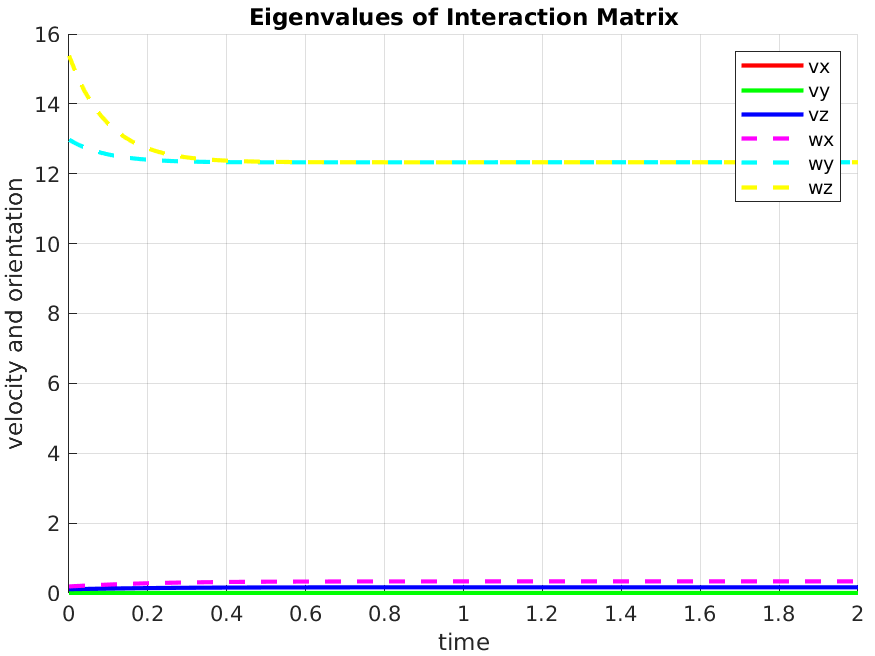
\includegraphics[height=1.2in]{../results/Demo1-eignen.png}
            \subcaption{Eignevalues}
                 \end{subfigure}%
         \begin{subfigure}[b]{0.32\textwidth}
                \centering
                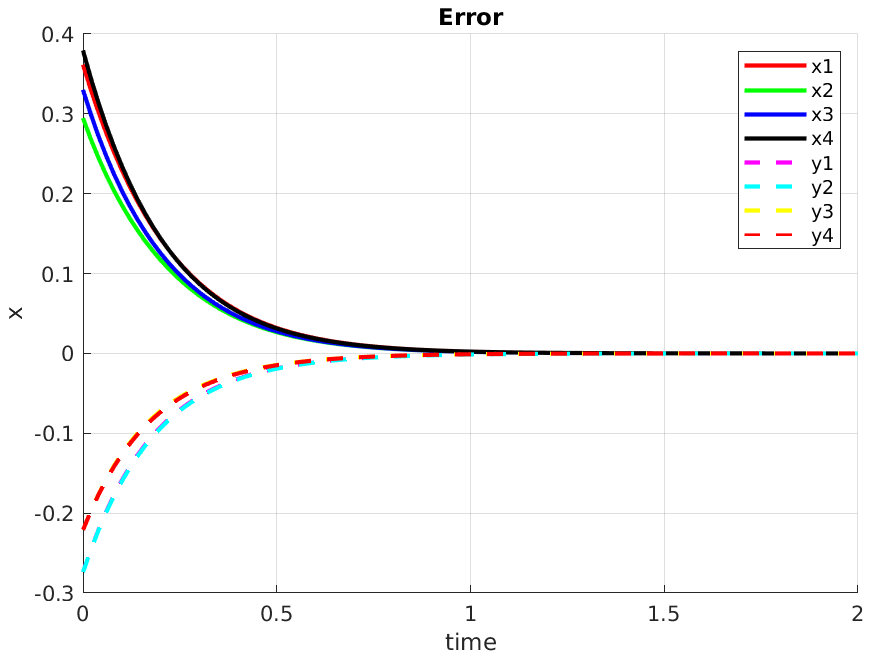
\includegraphics[height=1.2in]{../results/Demo1-error.png}
            \subcaption{Errors}
                 \end{subfigure}%
         \caption{Simple case : Observable pattern, the control law.}
        \label{fig:demo1}
\end{figure}
%\FloatBarrier
From the simulation results on Figure~\ref{fig:demo1} on page~\pageref{fig:demo1}, we observe that the camera follows a very good and straight path. The velocity is getting smaller and smaller as we aproaching the target. 
We notice that the interactiom matrix have some very high eigenvalues and some very small ones. So the DoF of the eigenvalues with big values is the only ones that drives the control of the system.
\subsubsection{Loosing Features: 3 points}
If we have only 3 points then we get 6 features witch is the minimum required. That not gurantes that we 
get a good solution in every case. Here the final camera location is almost correct. The movement have some instabilities, but that is expected due to the poorness interaction matrix. The simulation results is given at Figure~\ref{fig:demo2} on page~\pageref{fig:demo2}. The matlab code is on file \texttt{Demo2.m}.
\begin{figure}[tb!]
                 \begin{subfigure}[b]{\textwidth}         
                \centering
                 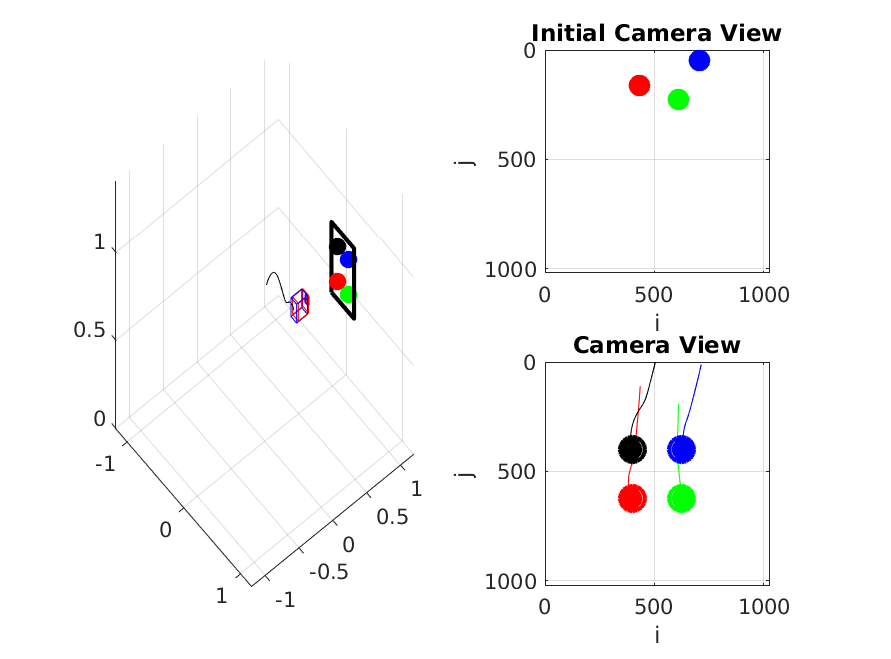
\includegraphics[width=13cm]{../results/Demo2-simulation.png}
             \caption{The camera motion}
             \vspace{8pt}
                 \end{subfigure}
         \begin{subfigure}[b]{0.32\textwidth}
                \centering
                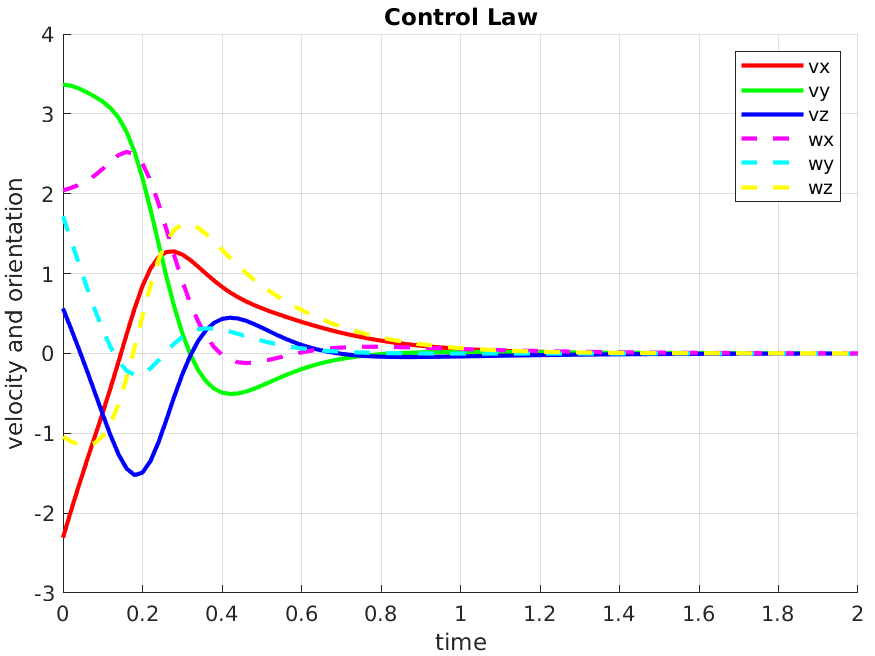
\includegraphics[height=1.2in]{../results/Demo2-control-law.png}
            \subcaption{Control Law}
                 \end{subfigure}
         \begin{subfigure}[b]{0.2\textwidth}
                \centering
                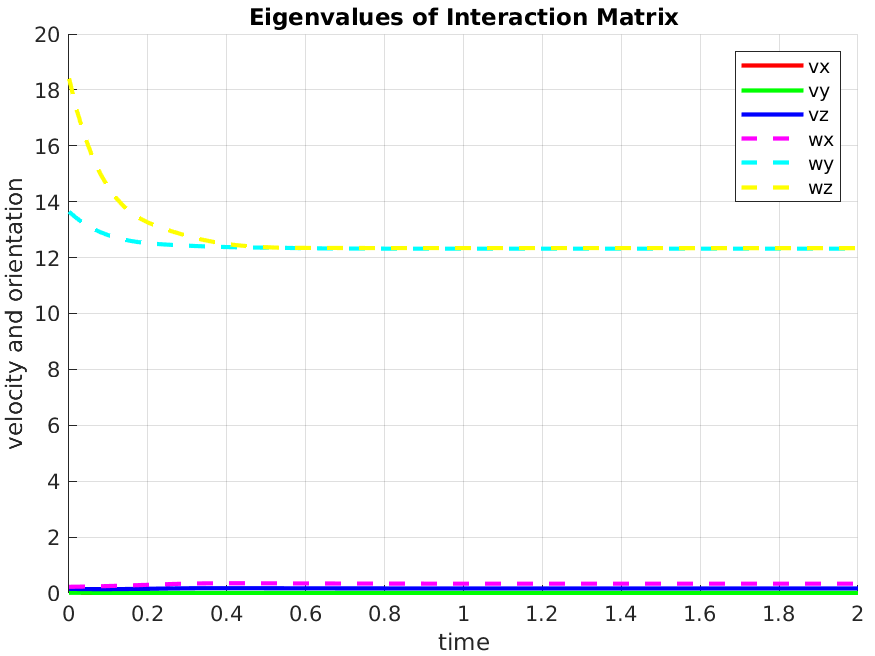
\includegraphics[height=1.2in]{../results/Demo2-eignen.png}
            \subcaption{Eignevalues}
                 \end{subfigure}%
         \begin{subfigure}[b]{0.32\textwidth}
                \centering
                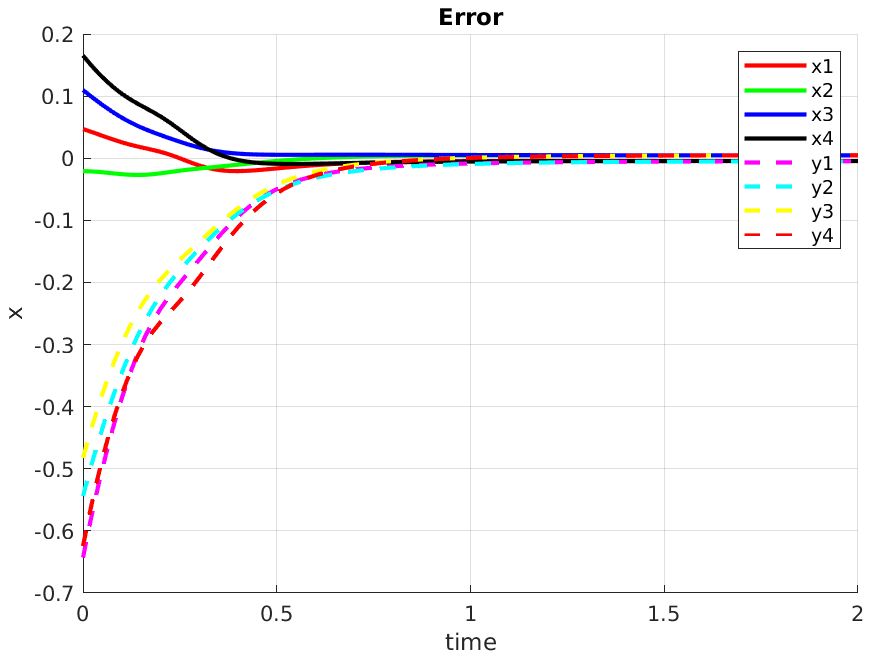
\includegraphics[height=1.2in]{../results/Demo2-error.png}
            \subcaption{Errors}
                 \end{subfigure}%
         \caption{Using 3 features : Observable pattern, the control law.}
        \label{fig:demo2}
\end{figure}
\subsubsection{Loosing Features: only 3 points}
In this experiment we track only 3 points, even if all points are presented on the camera. The camera motion is far away from ideal, it even goes behind the scene, increasing the error, but it finally manage to get a good solution. 
The simulation results is given at Figure~\ref{fig:demo2-3} on page~\pageref{fig:demo2-3}. The matlab code is on file \texttt{Demo2\_3var.m}.
\begin{figure}[tb!]
                 \begin{subfigure}[b]{\textwidth}         
                \centering
                 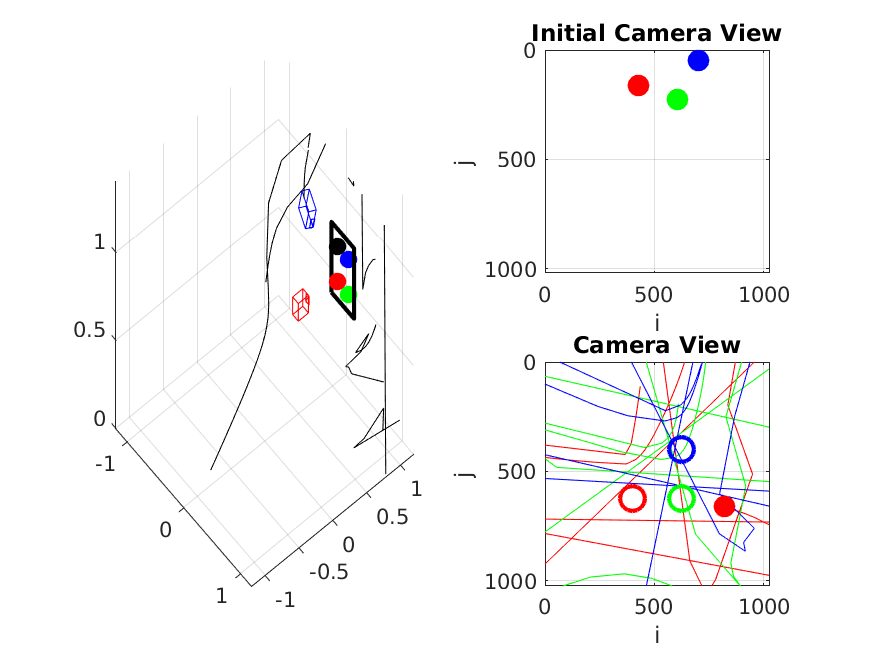
\includegraphics[width=13cm]{../results/Demo2-3-simulation.png}
             \caption{The camera motion}
             \vspace~
                 \end{subfigure}
         \begin{subfigure}[b]{0.32\textwidth}
                \centering
                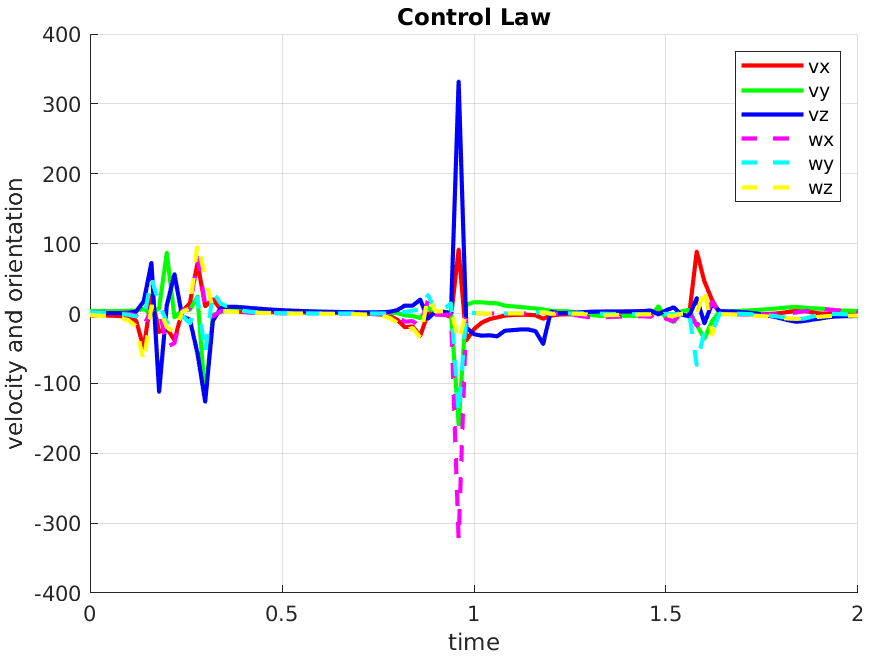
\includegraphics[height=1.2in]{../results/Demo2-3-control-law.png}
            \subcaption{Control Law}
                 \end{subfigure}
         \begin{subfigure}[b]{0.2\textwidth}
                \centering
                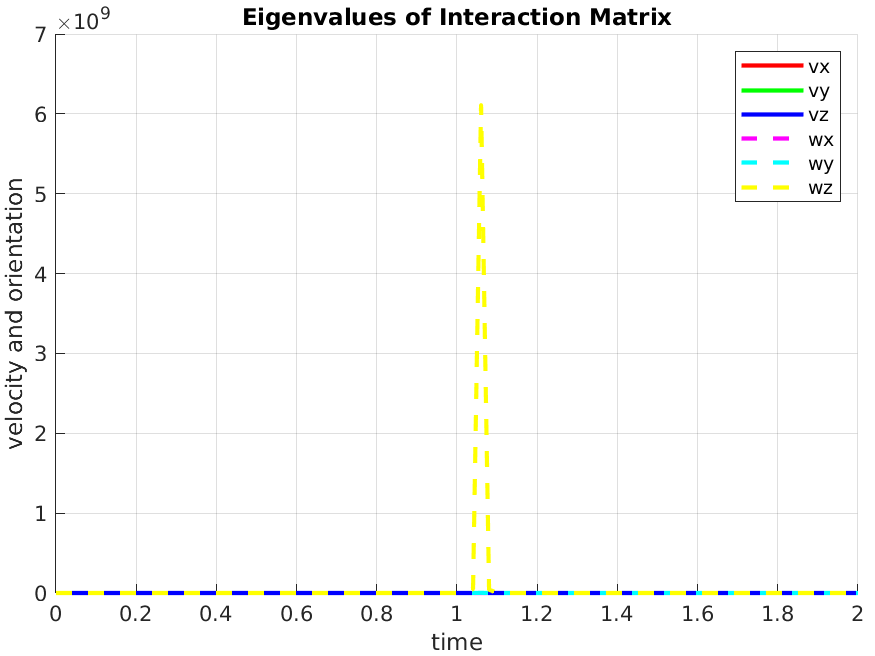
\includegraphics[height=1.2in]{../results/Demo2-3-eignen.png}
            \subcaption{Eignevalues}
                 \end{subfigure}%
         \begin{subfigure}[b]{0.32\textwidth}
                \centering
                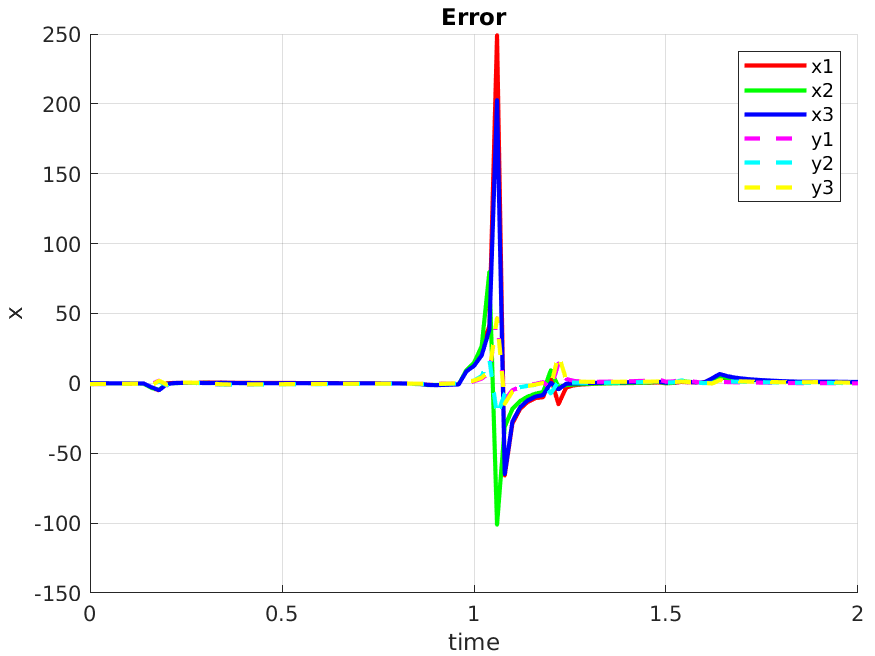
\includegraphics[height=1.2in]{../results/Demo2-3-error.png}
            \subcaption{Errors}
                 \end{subfigure}%
         \caption{Using only 3 features : Observable pattern, the control law.}
        \label{fig:demo2-3}
\end{figure}
\subsubsection{Loosing Features: 2 points}
By using only 2 point we get better results. That was not expected, but that is because of the 
initial view have 2 lines that is directed connected with the target lines it was easy to get a 
very smooth solution.  The simulation results is given at Figure~\ref{fig:demo3} on page~\pageref{fig:demo3}.  The matlab code is on file \texttt{Demo3.m}.
\begin{figure}[tb!]
                 \begin{subfigure}[b]{\textwidth}         
                \centering
                 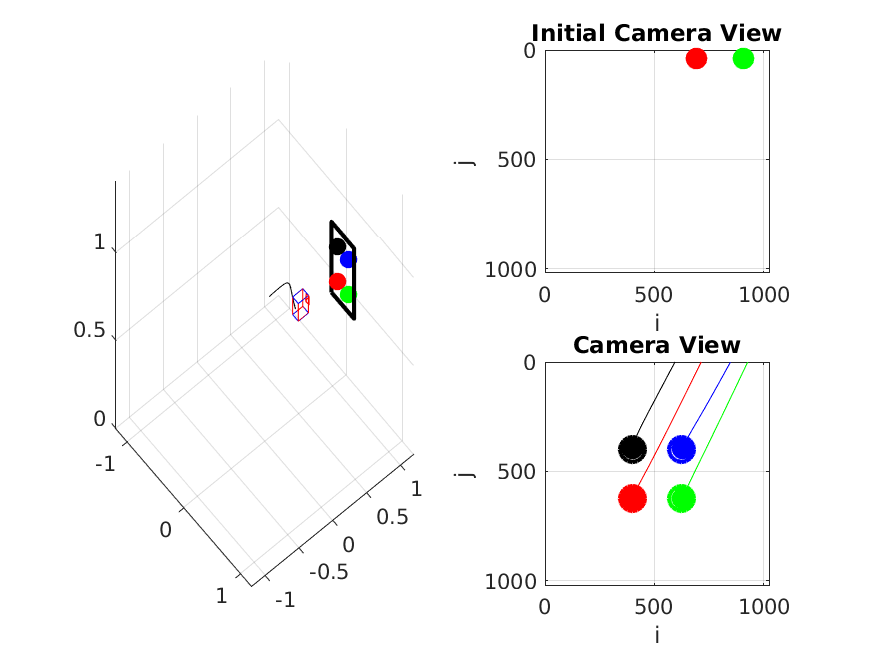
\includegraphics[width=13cm]{../results/Demo3-simulation.png}
             \caption{The camera motion}
             \vspace{8pt}
                 \end{subfigure}
         \begin{subfigure}[b]{0.32\textwidth}
                \centering
                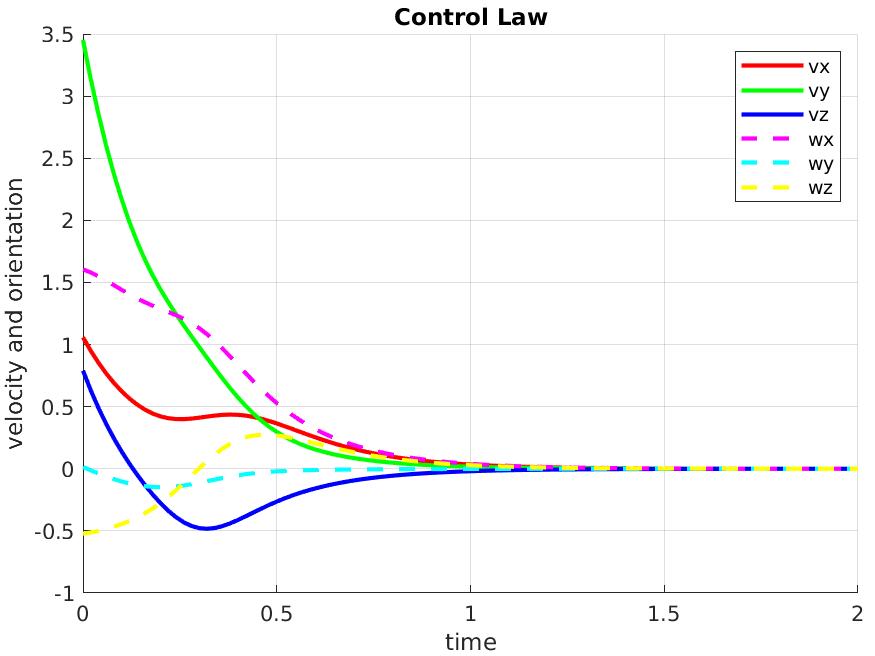
\includegraphics[height=1.2in]{../results/Demo3-control-law.png}
            \subcaption{Control Law}
                 \end{subfigure}
         \begin{subfigure}[b]{0.2\textwidth}
                \centering
                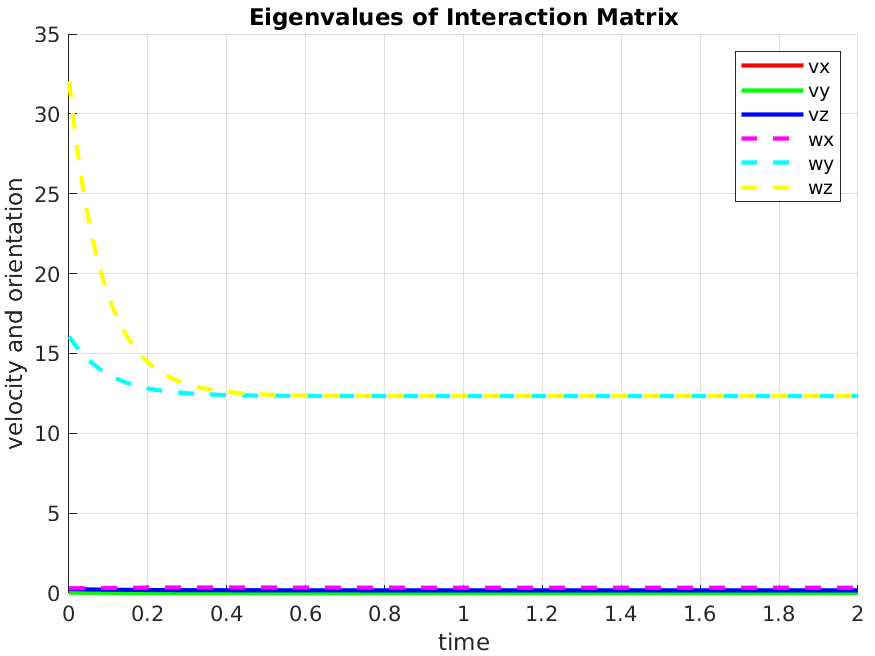
\includegraphics[height=1.2in]{../results/Demo3-eignen.png}
            \subcaption{Eignevalues}
                 \end{subfigure}%
         \begin{subfigure}[b]{0.32\textwidth}
                \centering
                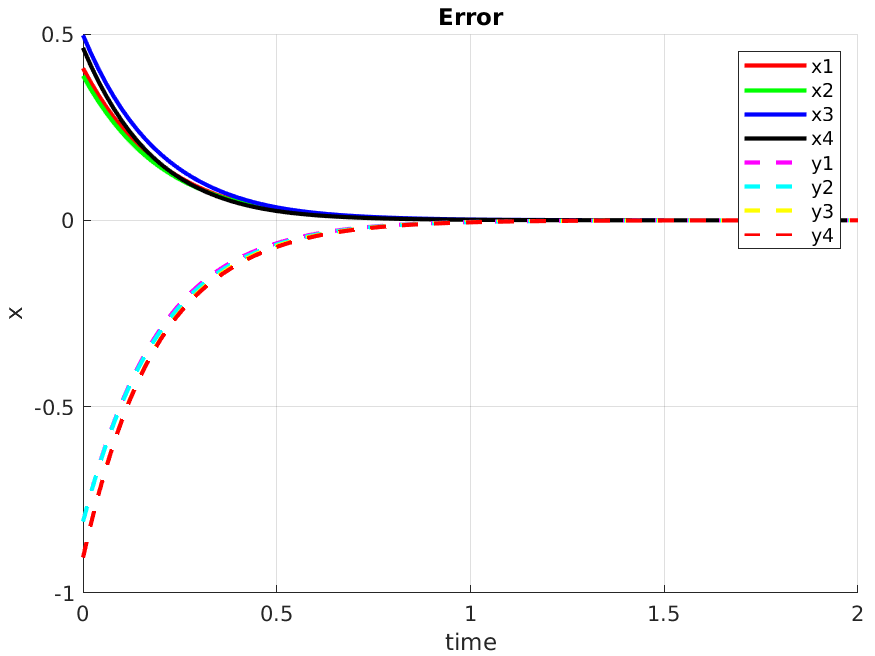
\includegraphics[height=1.2in]{../results/Demo3-error.png}
            \subcaption{Errors}
                 \end{subfigure}%
         \caption{Using 2 features : Observable pattern, the control law.}
        \label{fig:demo3}
\end{figure}
\subsubsection{The Coplanar Problem}
Here the human solution is just a rotation. But the solution to minimize the distances is to move the camera 
backwards as the error is decreasing. All the eignvalues are small in this case. The simulation results is given at Figure~\ref{fig:demo4} on page~\pageref{fig:demo4}. The matlab code is on file \texttt{Demo4.m}.
\begin{figure}[tb!]
                 \begin{subfigure}[b]{\textwidth}         
                \centering
                 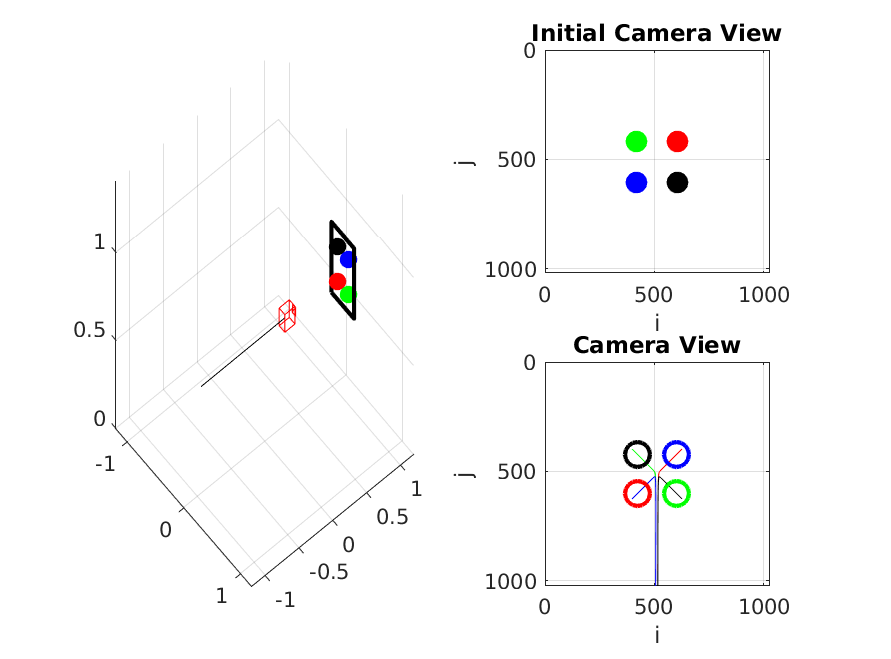
\includegraphics[width=13cm]{../results/Demo4-simulation.png}
             \caption{The camera motion}
			 \vspace{8pt}
                 \end{subfigure}
         \begin{subfigure}[b]{0.32\textwidth}
                \centering
                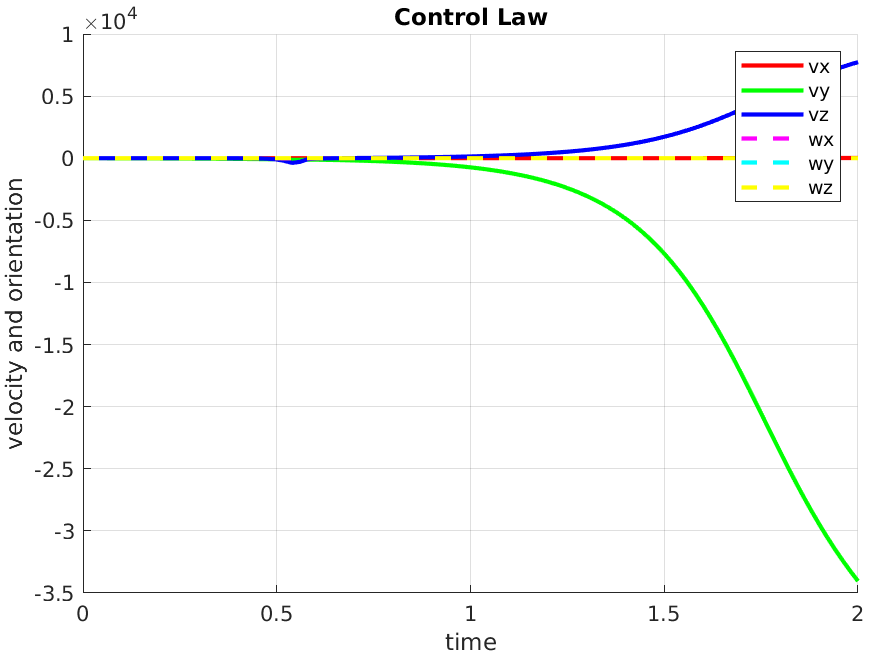
\includegraphics[height=1.2in]{../results/Demo4-control-law.png}
            \subcaption{Control Law}
                 \end{subfigure}
         \begin{subfigure}[b]{0.2\textwidth}
                \centering
                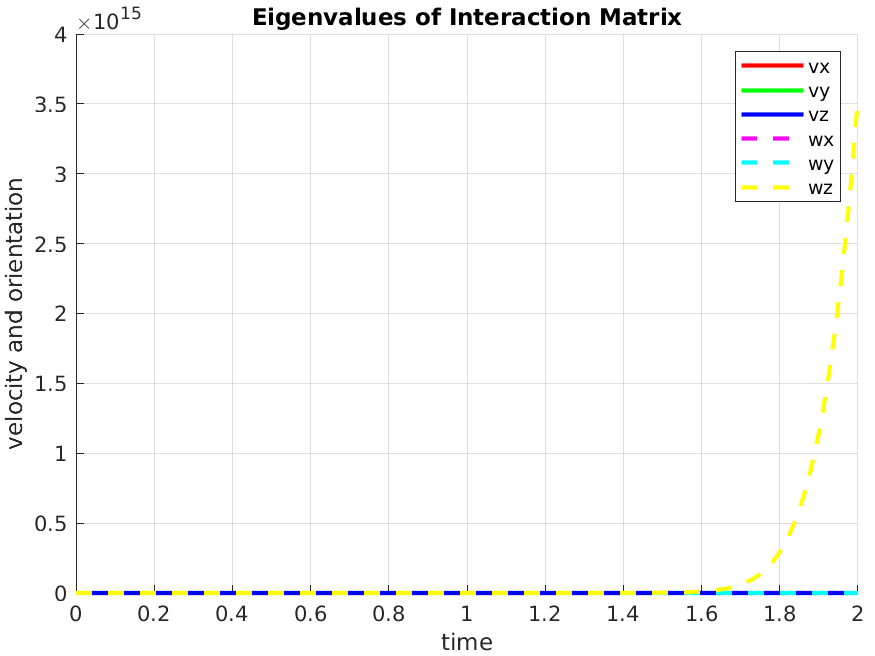
\includegraphics[height=1.2in]{../results/Demo4-eignen.png}
            \subcaption{Eignevalues}
                 \end{subfigure}%
         \begin{subfigure}[b]{0.32\textwidth}
                \centering
                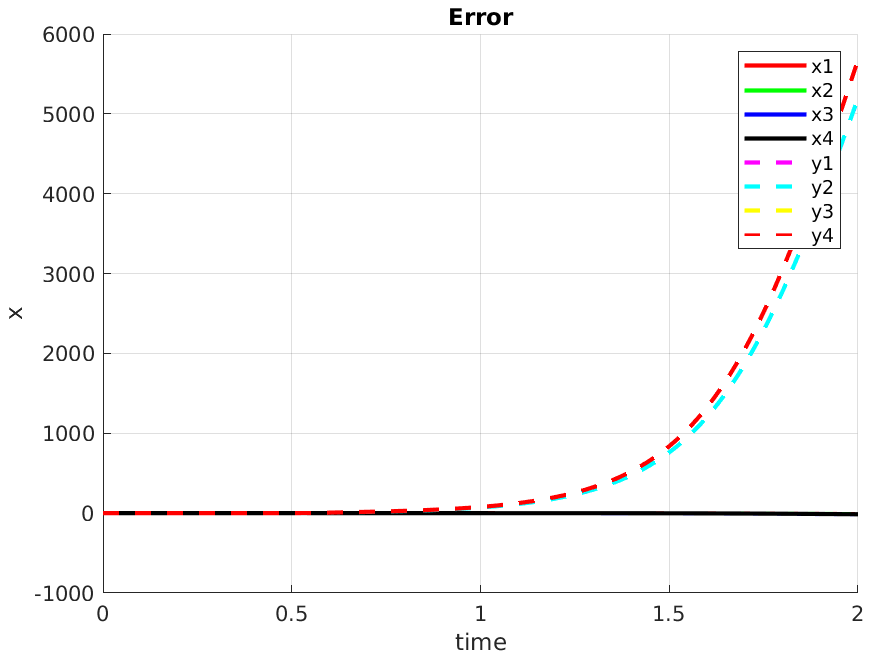
\includegraphics[height=1.2in]{../results/Demo4-error.png}
            \subcaption{Errors}
                 \end{subfigure}%
         \caption{The coplanar problem.}
        \label{fig:demo4} 
\end{figure}
\subsubsection{The Local Minimuma Problem}
The matrix $\mathbf{L} \widehat{\mathbf{L}_s^+} \in \Re^{k \times k}$ is at most of rank 6. With 4 points we 
have $k=8$ so it have a non-trivial null space. Thus configurations that corresponds to local minima exists.
In the setup of the experiment, the simulation runs into  a local minima and the control loop 
was unable to find a smooth path or a valid solution.
The simulation results is given at Figure~\ref{fig:demo5} on page~\pageref{fig:demo5}. The motion is shown in Figure~\ref{fig:vdemo5} on page~\pageref{fig:vdemo5}. The matlab code is on file \texttt{Demo5.m}.
\begin{figure}[tb!]
                 \begin{subfigure}[b]{\textwidth}         
                \centering
                 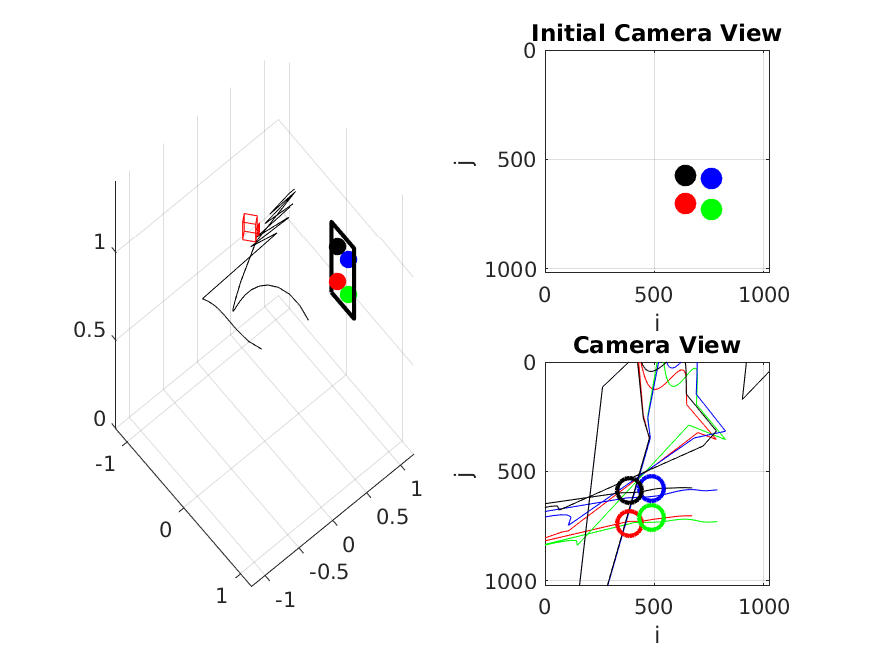
\includegraphics[width=13cm]{../results/Demo5-simulation.png}
             \caption{The camera motion}
             \vspace~
                 \end{subfigure}
         \begin{subfigure}[b]{0.32\textwidth}
                \centering
                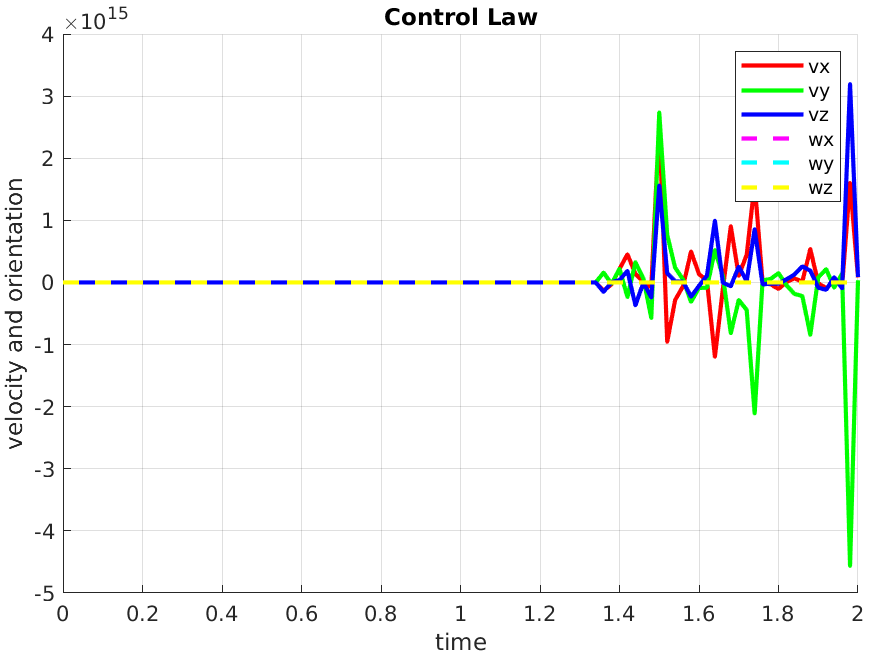
\includegraphics[height=1.2in]{../results/Demo5-control-law.png}
            \subcaption{Control Law}
                 \end{subfigure}
         \begin{subfigure}[b]{0.2\textwidth}
                \centering
                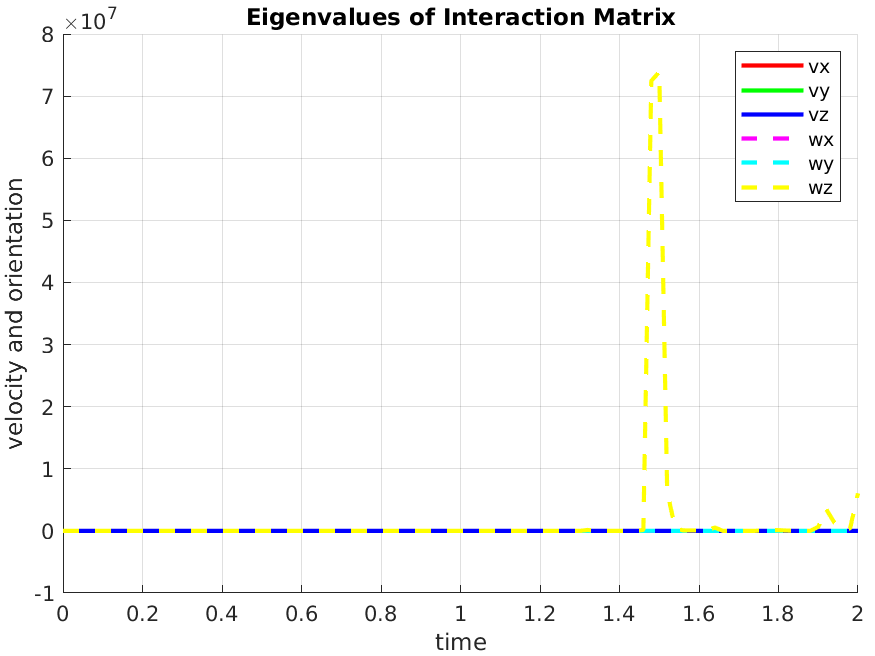
\includegraphics[height=1.2in]{../results/Demo5-eignen.png}
            \subcaption{Eignevalues} 
                 \end{subfigure}%
         \begin{subfigure}[b]{0.32\textwidth}
                \centering
                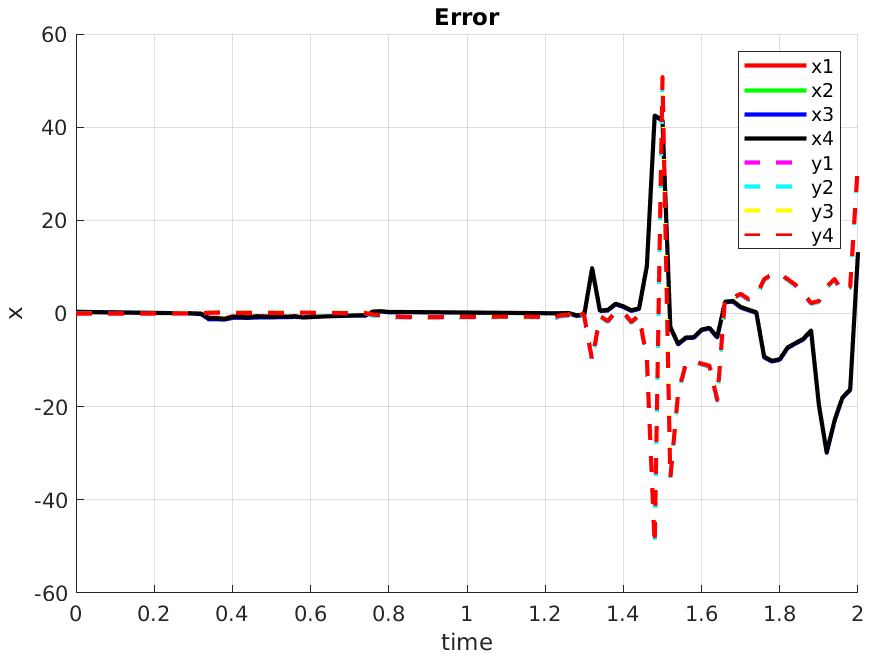
\includegraphics[height=1.2in]{../results/Demo5-error.png}
            \subcaption{Errors}
                 \end{subfigure}%
         \caption{The local minima problem.} 
        \label{fig:demo5} 
\end{figure}
\begin{figure}[tb!]
         \begin{subfigure}[b]{0.32\textwidth}
                \centering
                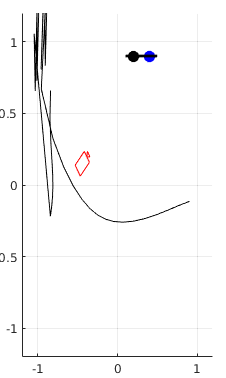
\includegraphics[height=1.2in]{../results/demo5-XY.png}
            \subcaption{XY view}
                 \end{subfigure}
         \begin{subfigure}[b]{0.2\textwidth}
                \centering
                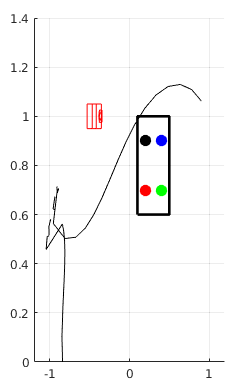
\includegraphics[height=1.2in]{../results/demo5-XZ.png}
            \subcaption{XZ view}
                 \end{subfigure}%
         \begin{subfigure}[b]{0.32\textwidth}
                \centering
                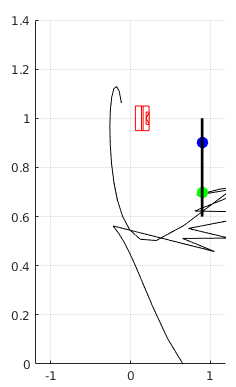
\includegraphics[height=1.2in]{../results/demo5-YZ.png}
            \subcaption{YZ View}
                 \end{subfigure}%
         \caption{The local minima problem: Motion Views} 
        \label{fig:vdemo5} 
\end{figure}
%\FloatBarrier
\begin{figure}[tb!]
         \begin{subfigure}[b]{0.32\textwidth}
                \centering
                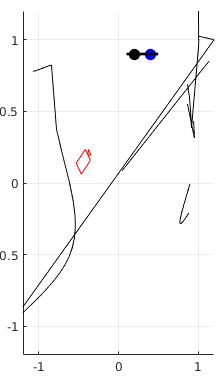
\includegraphics[height=1.2in]{../results/demo6-XY.png}
            \subcaption{XY view}
                 \end{subfigure}
         \begin{subfigure}[b]{0.2\textwidth}
                \centering
                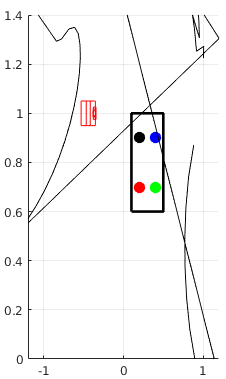
\includegraphics[height=1.2in]{../results/demo6-XZ.png}
            \subcaption{XZ view}
                 \end{subfigure}%
         \begin{subfigure}[b]{0.32\textwidth}
                \centering
                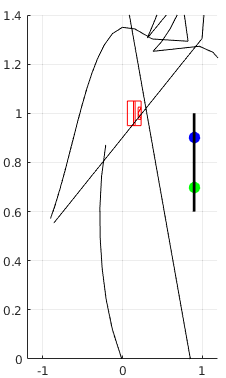
\includegraphics[height=1.2in]{../results/demo6-YZ.png}
            \subcaption{YZ View}
                 \end{subfigure}%
         \caption{The diverge problem: Motion Views} 
        \label{fig:vdemo6} 
\end{figure}
\subsubsection{The Diverge Problem}
Here a case where the control algorithm is diverging is demonstrated. The simulation results is given at 
Figure~\ref{fig:demo6} on page~\pageref{fig:demo6}. The motion is shown in Figure~\ref{fig:vdemo6} 
on page~\pageref{fig:vdemo6}. The matlab code is on file \texttt{Demo6.m}.
\begin{figure}[tb!]
                 \begin{subfigure}[b]{\textwidth}         
                \centering
                 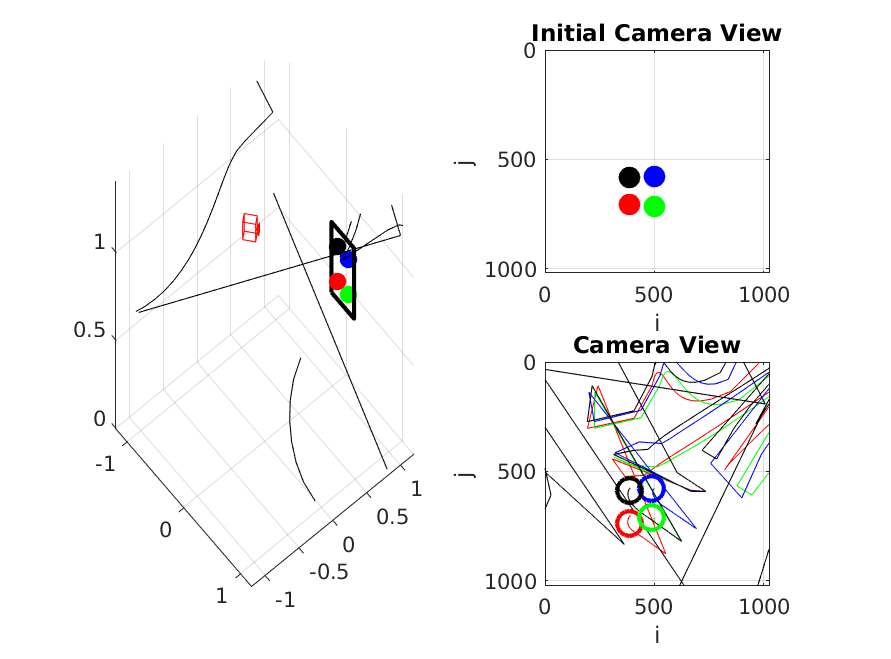
\includegraphics[width=13cm]{../results/Demo6-simulation.png}
             \caption{The camera motion}
             \vspace~
                 \end{subfigure}
         \begin{subfigure}[b]{0.32\textwidth}
                \centering
                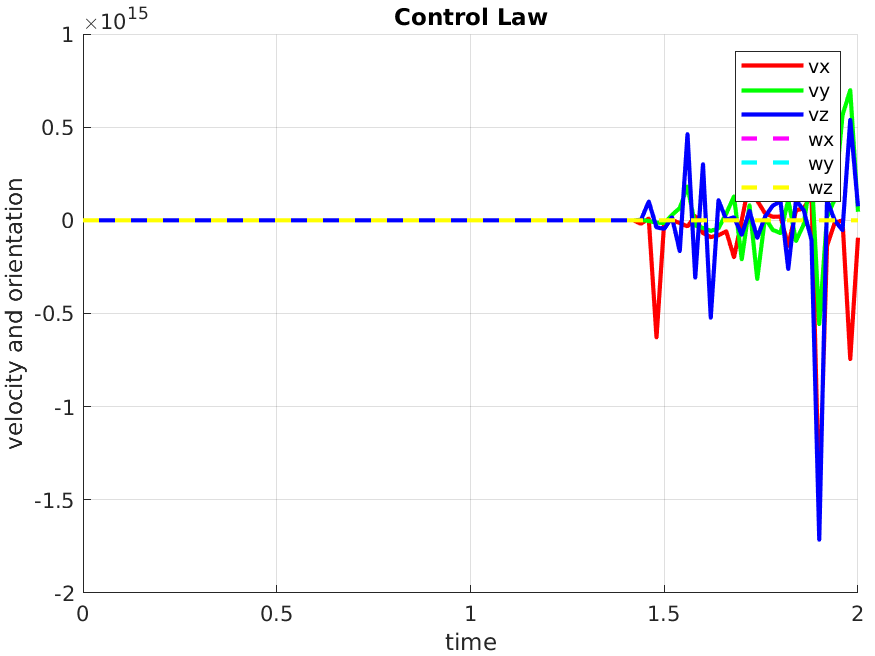
\includegraphics[height=1.2in]{../results/Demo6-control-law.png}
            \subcaption{Control Law}
                 \end{subfigure}
         \begin{subfigure}[b]{0.2\textwidth}
                \centering
                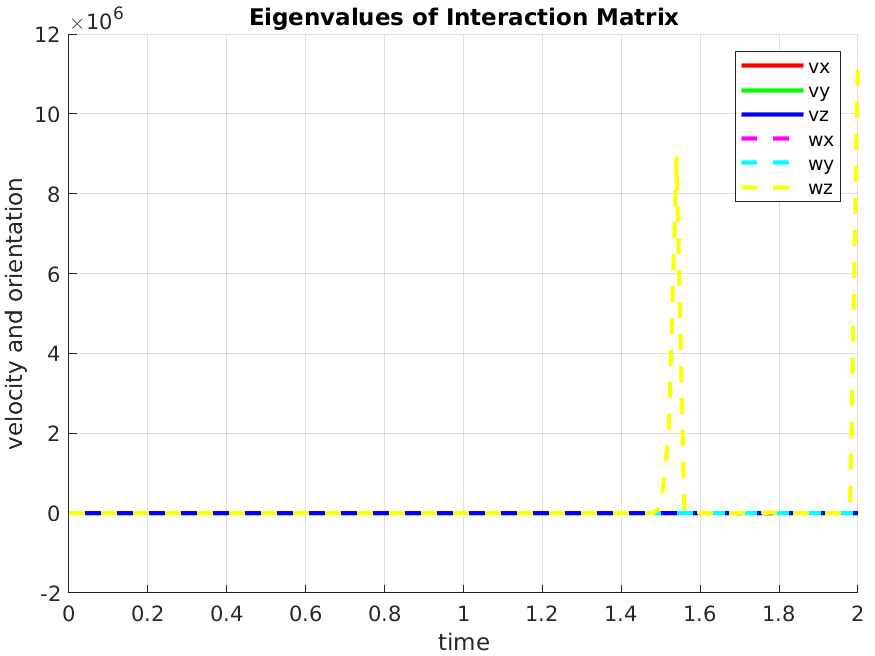
\includegraphics[height=1.2in]{../results/Demo6-eignen.png}
            \subcaption{Eignevalues}
                 \end{subfigure}%
         \begin{subfigure}[b]{0.32\textwidth}
                \centering
                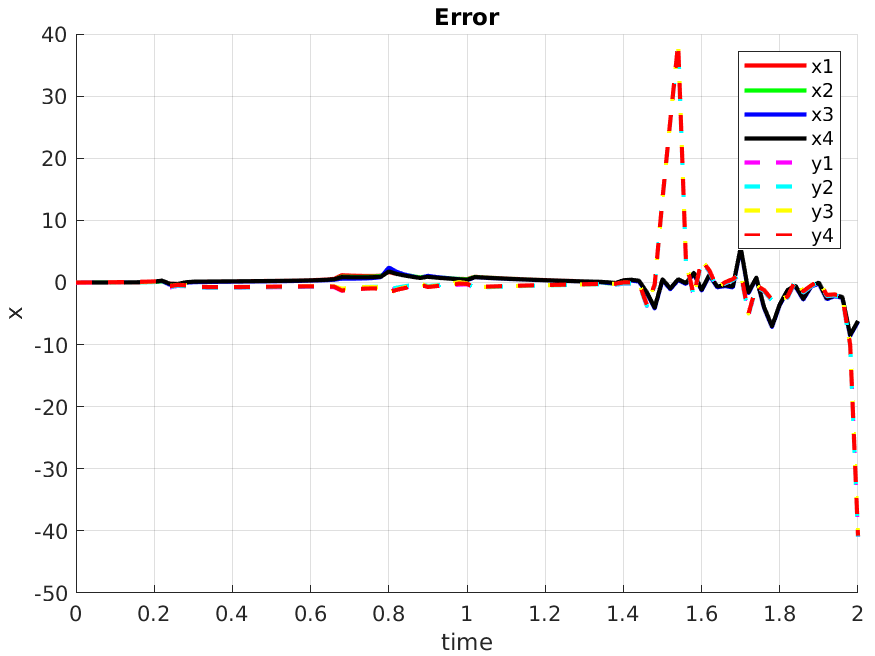
\includegraphics[height=1.2in]{../results/Demo6-error.png}
            \subcaption{Errors}
                 \end{subfigure}% 
         \caption{The diverge problem.} 
        \label{fig:demo6} 
\end{figure}
\FloatBarrier
\subsection{Position Based Visual Servoing} 
We want to move a camera from its current Cartesian pose to a desired Cartesian pose (see Figure~\ref{fig:pbvs} on page~\pageref{fig:pbvs}). We
assume that we can measure the Cartesian pose of the camera at every instant of time using a sensor.
\begin{figure}[tb!]
         \centering
         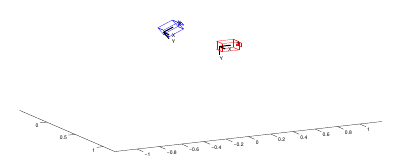
\includegraphics[width=13cm]{../images/PBVS-intro.png}
         \caption{Camera pose control. Blue camera shows the initial pose of the camera, and the red camera
shows the desired pose of the camera.
.}
        \label{fig:pbvs}
\end{figure}
\subsubsection{Matlab simulation}
Here the camera pose at each time step is known. The movement of the camera is very smooth and it reach the desired location without problems. The simulation results is given at Figure~\ref{fig:pbvsr} on page~\pageref{fig:pbvsr}. The matlab code is on file \texttt{Demo1PBVS.m}.
\begin{figure}[bt!] 
         \begin{subfigure}[b]{0.32\textwidth}
                \centering
                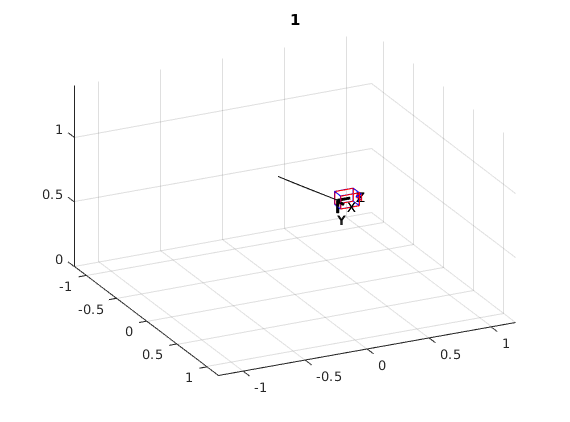
\includegraphics[height=1.2in]{../results/PBVS3.png}
            \subcaption{Camera movement}
                 \end{subfigure}
         \begin{subfigure}[b]{0.2\textwidth}
                \centering
                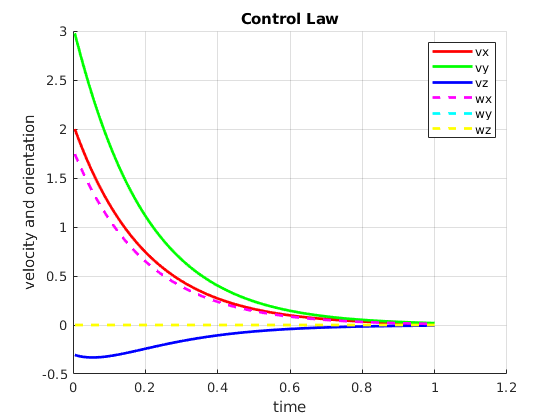
\includegraphics[height=1.2in]{../results/PBVS2.png}
            \subcaption{Errors over time}
                 \end{subfigure}%
         \begin{subfigure}[b]{0.32\textwidth}
                \centering
                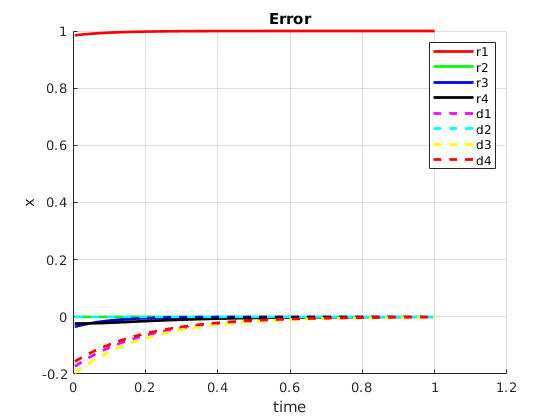
\includegraphics[height=1.2in]{../results/PBVS1.png}
            \subcaption{Camera control law}
                 \end{subfigure}%
         \caption{Position Based Visual Servoing} 
        \label{fig:pbvsr} 
\end{figure}
\section{Conclusions}
The IBVS is a useful for controlling a robot using visual information. But as it it does not take into
account the position of the camera in its 3D world and have many stability issues.   When  only  one
image  is  used,  even  small  errors  in  the  image  measurements can lead to errors in the pose that can impact significantly the accuracy of the system.
The  PBVS use no visual information.  Since  the  control  scheme  imposes  a  behaviour  of  $\mathbf{s}$ which  is  here  expressed  in  the  Cartesian  space,  it  allows  the camera  to  follow  theoretically  an  optimal  trajectory  in  that space  but  generally  not  in  the  image  space. 
Even if the two basic approaches presented   give in practice satisfactory results in most cases, their
respective shortcomings have led to many works and improvements. Clearly a combination of both methods will give us better results.
\subsection{MatlabCode}
The code of this project is on Github repository \url{https://github.com/jtsagata/VisualServoingLab}.
\FloatBarrier
\section{Bibliography}
\begin{thebibliography}{9}
\bibitem{notes}
  \emph{Lecture and lab notes}.
\bibitem{Farrokh}
  Farrokh Janabi-Sharifi,
  Visual Servoing : Theory and applications, Chapter 15 (book unknown)
\bibitem{Chaumette1}
  F. Chaumette, S. Hutchinso,
  \emph{ Visual Servo Control, Part I: Basic Approaches}.
EEE Robotics and Automation Magazine, 13(4):82-90, December 2006.
\bibitem{Chaumette12}
  F. Chaumette, S. Hutchinson,
  \emph{Visual Servo Control, Part II: Advanced Approaches}.
  Addison Wesley, Massachusetts,
IEEE Robotics and Automation Magazine, 14(1):109-118, March 2007
\bibitem{Hutchinson}
 S. A. Hutchinson, G. D. Hager, and P. I. Corke,
\emph{ A tutorial on visual servo control}.
        IEEE Trans. Robot. Automat., 12(5):651—670, Oct. 1996.
\bibitem{Corke}
 P. I. Corke,
\emph{ Robotics, Vision and Control: Fundamental Algorithms in MATLAB}.
        Springer, 2013.
\end{thebibliography}
\clearpage 
\end{document} % NOTHING AFTER THIS LINE IS PART OF THE DOCUMENT
